\section{The Main Project}
\noindent
The core of the internship was centered around the design and development of an \textbf{Intern Management Platform}, an internal solution for \textbf{VOID Digital Agency}. The goal was to streamline the onboarding, tracking, evaluation, and reporting processes for interns, while showcasing modern development practices such as \textbf{headless CMS architecture}, \textbf{agile workflows}, and \textbf{continuous deployment pipelines}.

\medskip

\noindent
Although the initial division of tasks assigned me the responsibility of \textbf{designing the UX/UI} of the platform, \textbf{meeting with the head of VOID} to align with the business needs, \textbf{developing the frontend} using \textbf{React/Next.js}, \textbf{integrating it with a headless Drupal backend}, in practice we adopted a \textbf{dynamic collaboration system}.  
This system was based on \textbf{weekly shifts}, allowing both my colleague and me to contribute to all aspects of the platform: including frontend, backend, DevOps infrastructure, and CI/CD pipelines.  
This approach ensured a complete understanding of the entire digital ecosystem and promoted continuous knowledge sharing.

\subsection{Training Phase at VOID}
\noindent
Before engaging in the development of the Intern Management Platform, VOID Digital Agency organized a two and a half months internal training phase. This training covered the main technologies and methodologies required for the project, including Headless Drupal CMS, Next.js development, Agile workflows, DevOps practices, and CI/CD pipelines.  
The training ensured that all team members were aligned on technical standards and development best practices.  
% The following Gantt chart illustrates the timeline of this initial training phase:

% \begin{figure}[H]
%     \centering
%     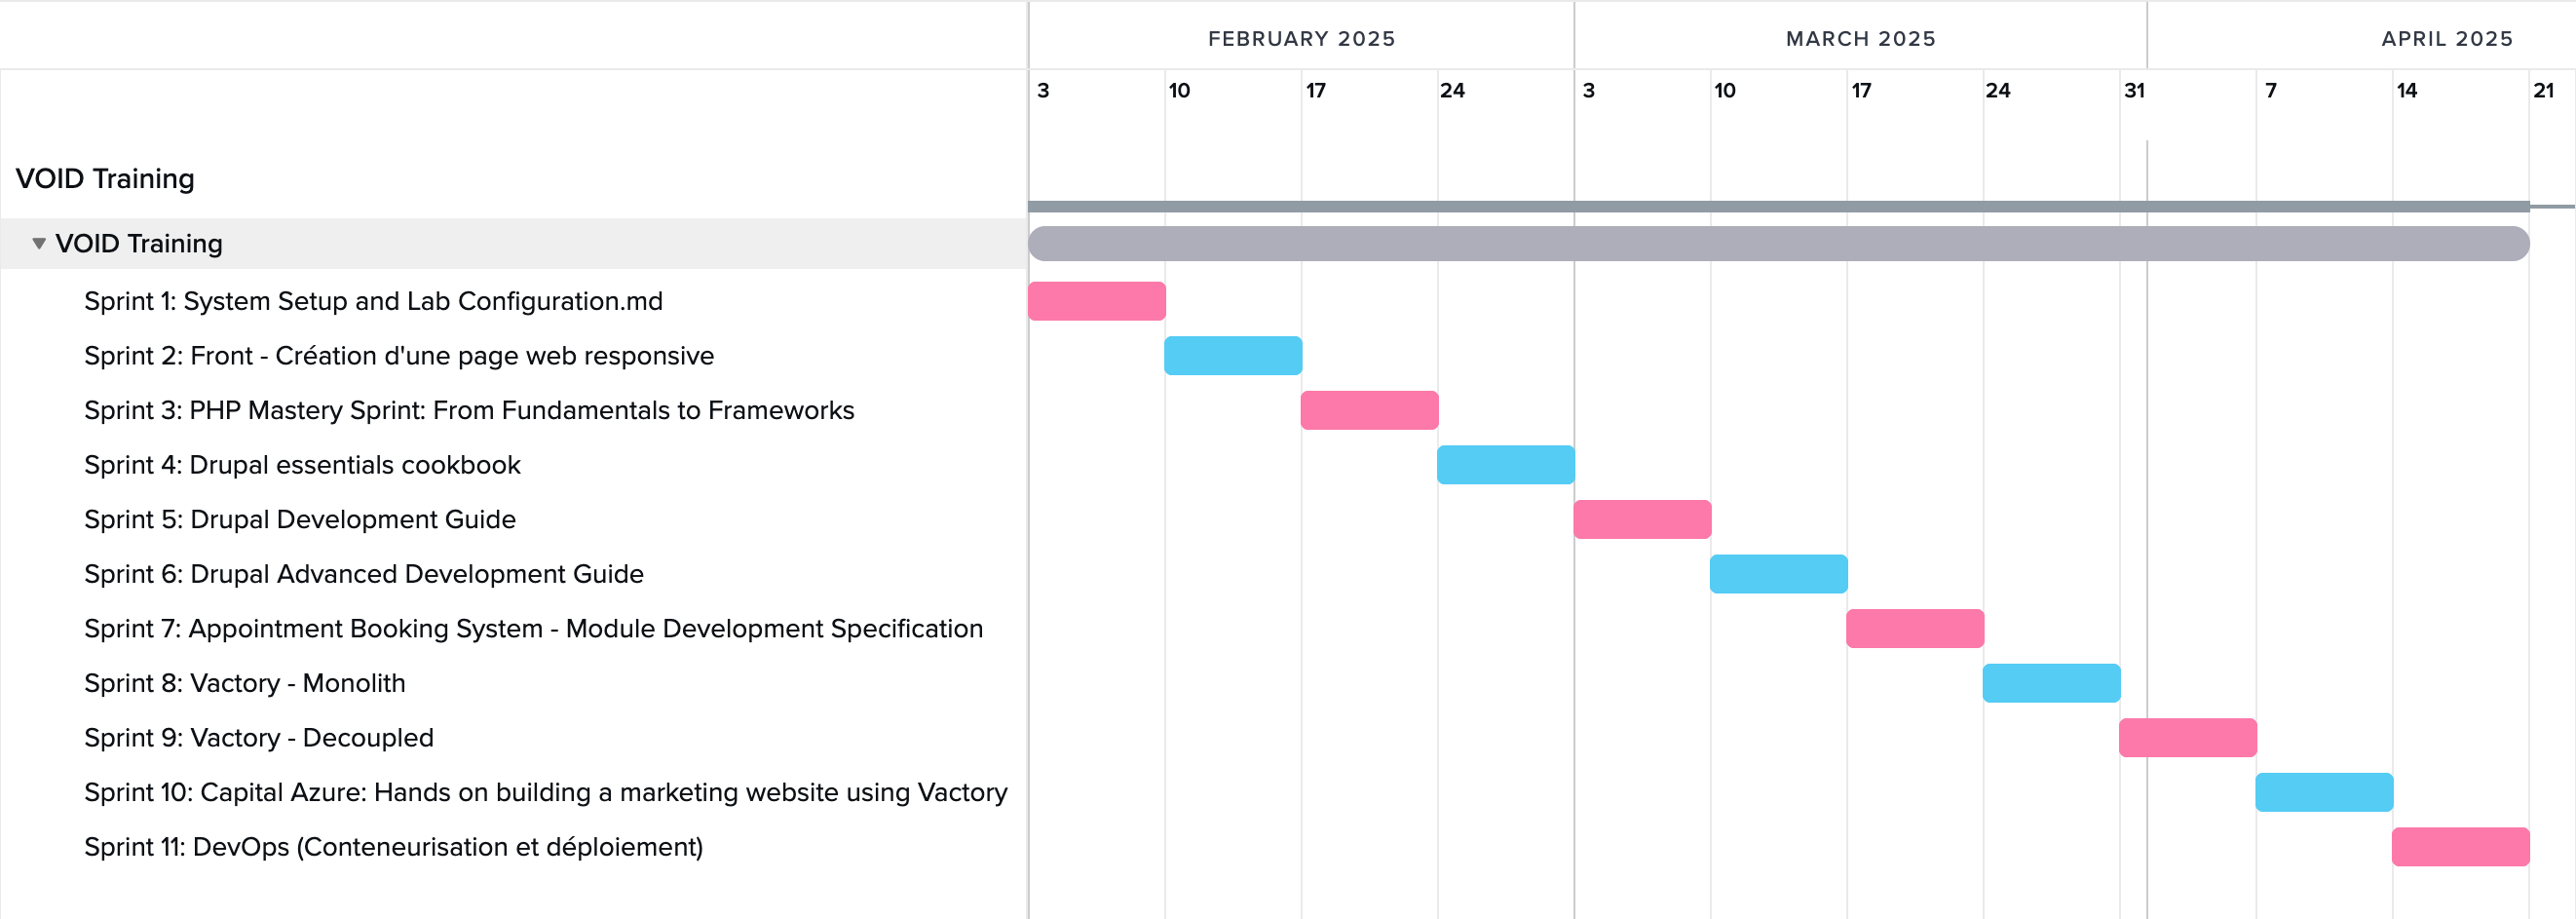
\includegraphics[width=0.9\textwidth]{images/training-ganttChart.png}
%     \caption{Gantt Chart of the Training Phase at VOID}
% \end{figure}

\medskip
\noindent
This foundational training was crucial in building the necessary skills and preparing for the successful delivery of the project.

% Then continue the real project parts
\subsection{Problematic}
\noindent
VOID, like many digital agencies, manages a significant number of interns each year across various departments — development, UX/UI design, marketing, project management, and more.  
The traditional intern management relied heavily on manual tracking, disconnected communication channels, and dispersed data storage (Excel sheets, emails, local files), resulting in several critical issues:
\begin{itemize}
  \item Lack of centralized data regarding intern profiles, progress, and evaluations.
  \item Difficulty for supervisors to monitor onboarding status, project allocations, and intern deliverables.
  \item Absence of real-time reporting on intern activity, skill assessments, and final evaluations.
  \item Inconsistencies and inefficiencies in document generation (attestation letters, certificates, evaluation reports).
\end{itemize}

\medskip

\noindent
These limitations not only increased administrative workload, but also slowed decision-making and reduced the overall quality of intern experiences at VOID.  
A scalable, structured, and automated solution was thus necessary to improve operational efficiency and enhance the agency's capacity to support and evaluate its interns effectively.

\medskip

\subsection{Objectives}
\noindent
The Intern Management Platform was designed with the following main objectives:

\begin{itemize}
  \item \textbf{Centralization:} Create a unified platform to store and manage all intern-related data, from applications to evaluations.
  \item \textbf{Automation:} Automate key workflows such as onboarding tracking, evaluation form generation, and certificate issuance.
  \item \textbf{Scalability:} Build the system with a scalable architecture using \textbf{headless Drupal} and \textbf{Next.js}, ensuring future extensibility (adding new modules like training plans, skill assessments, etc.).
  \item \textbf{User Experience:} Offer an intuitive and efficient user experience for both \textbf{candidates} and \textbf{employers} through a clean and responsive UX/UI design.
  \item \textbf{Monitoring and Reporting:} Equip supervisors with real-time dashboards and reporting tools to track intern progression, performance, and document generation.
  \item \textbf{DevOps and CI/CD:} Ensure that the deployment of the platform follows best practices with a robust CI/CD pipeline, enabling automated testing, building, and deployment processes.
\end{itemize}

\medskip

\noindent
While I was initially focused on the UX/UI design and the development of the \textbf{Candidate Space} (frontend and backend), thanks to our rotation system, I actively contributed across all project dimensions, including DevOps setup, backend integrations, and global system testing.

\subsection{Proposed Solution}
\noindent
To meet the objectives and address the problems identified, the proposed solution was to design and build a comprehensive \textbf{Intern Management Platform} structured into three interconnected modules:

\begin{itemize}
  \item \textbf{Website:} A public-facing site aimed at presenting VOID's internship program, its philosophy, stages, and benefits. It includes a \textbf{Call-to-Action (CTA)} allowing candidates to apply directly. This site serves as the primary entry point to attract and engage potential interns.

  \item \textbf{Candidate Space (Espace Candidat):} A dedicated portal where candidates can:
  \begin{itemize}
    \item Browse internship offers posted by VOID.
    \item Apply to internships by submitting personal information, CVs, cover letters, and any other required documents.
    \item Track the status of their application (in progress, accepted, rejected).
    \item Participate in tests and interviews conducted as part of the recruitment process.
  \end{itemize}
  This space was built using \textbf{React/Next.js} for the frontend and connected to a \textbf{headless Drupal CMS} backend serving structured data via APIs, ensuring flexibility, scalability, and performance.

  \item \textbf{Training Space (Espace Formation):} Once accepted, interns gain access to this space, modeled after modern online learning platforms such as Coursera. Here, they can:
  \begin{itemize}
    \item Follow predefined training roadmaps aligned with VOID's standards.
    \item Access courses, videos, assignments, and learning materials.
    \item Complete projects and quizzes over a three-month structured program.
    \item Monitor their own progression through dashboards and receive feedback from supervisors.
  \end{itemize}
  This module supports VOID's mission of continuous learning and ensures that interns are fully prepared for their assigned roles.
\end{itemize}

\medskip

\noindent
The technical implementation was based on a \textbf{headless architecture}, where Drupal managed the content models, permissions, and workflows, while the frontend was fully decoupled, using \textbf{Next.js} for server-side rendering and dynamic interaction.  
The backend exposed structured data through \textbf{JSON:API} endpoints, and all user interactions were designed to be smooth and reactive, respecting the best practices of modern UX/UI design.

\medskip

\noindent
Additionally, the entire project was deployed using a full \textbf{CI/CD pipeline} to automate testing, building, and production delivery.

\medskip

\noindent
Although my initial responsibilities mainly covered the \textbf{UX/UI design}, \textbf{meetings with the head of VOID}, the development of the \textbf{Candidate Space} (frontend and headless backend integration), our \textbf{rotation system} allowed me to work on all areas, including the \textbf{Training Space} and infrastructure tasks.  
This dynamic approach enhanced my skills across the complete technological stack and provided a holistic understanding of the system lifecycle.

